\section{Results \& Discussion}

The training process for each model was evaluated using a cumulative average of the score, as illustrated in Fig. \ref{fig: Training curve - Infinite} and Fig. \ref{fig: Training curve - Finite}. The infinite situation converged after approximately '' iterations, which is a considerable amount less than for the finite situation, with '' iterations. This was a direct result of the difference in state spaces, where the finite situation required more iterations to converge its larger q-table. The two systems converged to similar cumulative average scores. This is notable because it indicates that the probability dimension in the finite q-table effectively managed inconsistent probabilities. 

\begin{figure}[ht] 
    \centering
    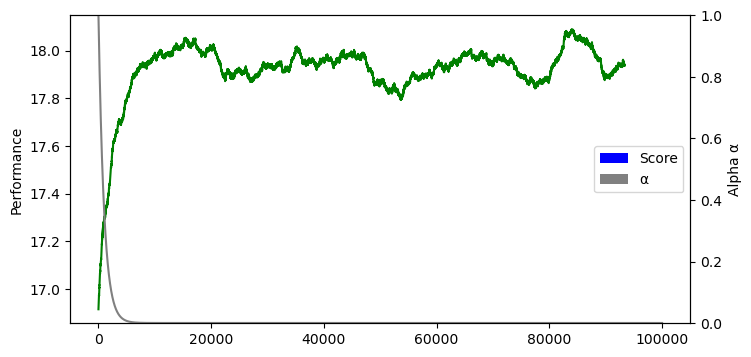
\includegraphics[width=\singlefigure]{figures/infinite_training_curve.png}
    \caption{Agent's training curve and learning rate in the infinite situation}
    \label{fig: Training curve - Infinite} 
\end{figure}



\begin{figure}[ht] 
    \centering
    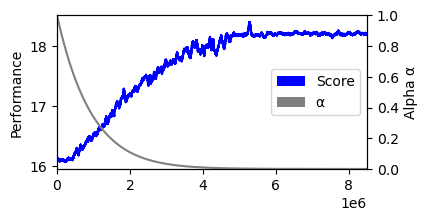
\includegraphics[width=\singlefigure]{figures/finite_training_curve.png}
    \caption{Agent's training curve and learning rate in the finite situation.}
    \label{fig: Training curve - Finite} 
\end{figure}

The expected value of the next card in the infinite situation is \(6.54\), which is approximately the difference between 21 and its converged value. This validates the system, because the algorithm wants an even split of probability????

Stick values in each Q-table quickly converged to their value squared, as defined by equation \ref{reward}, the reward equation. This was because the agent saw no future maximum value. In contrast, the Hit values in the Q-table took longer to converge. This was due to their probabilistic nature, in which, enough cards had to be dealt for 

Optimal hyperparameters were selected for each situation via a grid-search approach, in which a selection of hyperparameters were tested and compared. Following this, Gamma \(\gamma\) was defined as 1 because this would ensure that the future maximum reward was as valuable as current reward. Similarly, an optimum Epsilon \(\epsilon\) was defined as 0.1. Alpha decay rates, however, differed between the two systems, with infinite using an optimum of 0.01 and finite using 0.08. 

The resulting optimal policies \(\pi^*\) are plotted in Fig. \ref{fig: Optimal policy - Infinite} for the infinite situation and Fig. \ref{fig: Optimal policy - Finite} for the finite situation. The infinite policy hits until 14 with no unused ace, and until 17 with an unused ace, which differs from the statistical stance of sticking on 17 irrespective of the held cards. The differences between this policy and the statistical optimum is due to the squared reward defined in \ref{eq: Score} and the absence of an active dealer. This drives the agent to be adverse to risk, preferring to receive a definitive reward. 

\begin{figure}[ht]
    \centering
    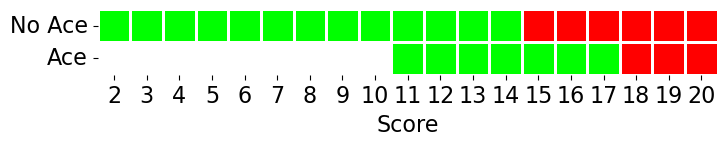
\includegraphics[width=\singlefigure]{figures/infinite_optimal_policy.png}
    \caption{Optimal policy for the infinite situation, with green indicating hit, and red indicating stick.}
    \label{fig: Optimal policy - Infinite} 
\end{figure}

The finite policy, in contrast, did not fully converge due to some states being very rarely entered, such as a 30\% chance of losing with a current score of 20. These values are missing in the respective Q-table. Despite this, commonly entered states developed a policy exhibiting logical patterns - sticking when loss is likely, and hitting when loss is unlikely. Additionally, the policy follows a diagonal split. This is because with a low card count, there is a higher future maximum value, meaning that even with a high chance of losing, the agent is willing to be 

The rarity of entering regions in the top right and bottom left was due to 
The inequality between these areas was due to \(4\times10\) valued cards.

\begin{figure}[ht]
    \centering
    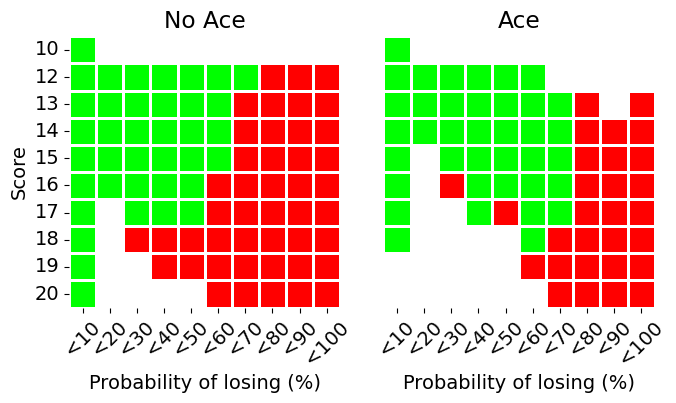
\includegraphics[width=\singlefigure]{figures/finite_optimal_policy.png}
    \caption{Optimal policy for the finite situation, with green indicating hit, and red indicating stick. This model was trained over 400000 iterations and 2 decks. Probability bins of 10\% increments are indicated accordingly. Missing policy points did not converge during training.}
    \label{fig: Optimal policy - Finite} 
\end{figure}

%To combat this issue, the rarely entered states could have been artificially entered, as this would have converged q-values irrespective of the agent's environment. 